\chapter{Prérequis et points d’attention pour le pilotage de projets d’automatisation via l’IA dans les archives}

\subsection{Des besoins métier multiples mais des cas d'usage à préciser}

Les paragraphes précédents illustrent à quel point les besoins et possibilités en termes
d'automatisation sont nombreux chez les producteurs d'archives publiques.
Les services ont l'opportunité d'expérimenter avec l'IA. Il est plus aisé
d'obtenir des financements publics pour des projets qui utilisent des
technologies dans l'ère du temps. Les projets IA obtiennent d'autant
plus de financements dans le cadre de leur promotion par les états
mentionnée en première partie. Ce type de projets nécessite néanmoins une
réflexion approfondie en amont pour assurer un pilotage efficace et
garantir des résultats concrets.\newline

Tout d'abord, pour que ces projets impliquant du \emph{machine learning}
réussissent, ils doivent non seulement répondre à des besoins métier,
mais également avoir des cas d'utilisation bien précis. Le cas
d'utilisation ou cas d'usage est défini par Alistair Cockburn, expert en
\gls{agiles}, comme «~une description des séquences possibles
d\textquotesingle interactions entre un système en question et ses
acteurs externes, liées à un objectif particulier\footcite{cockburn_writing_2001}~» {[}Traduction libre{]}. L'informaticien suédois Ivar
Jacobson aurait été le premier à introduire des cas d'usage à la fin des
années 1960\footcite{cockburn_writing_2001}. C'est à partir des années
1980-1990 qu'ils ont été davantage formalisés. D'après Alistair
Cockburn, pour rédiger un cas d\textquotesingle utilisation efficace, il
faut commencer par définir clairement le périmètre du système et
identifier tous les acteurs et leurs objectifs. Il faut ensuite rédiger
le scénario de succès principal en décrivant chaque étape comme un
objectif atteint, puis ajouter les alternatives et les échecs possibles\footcite{cockburn_writing_2001}.
Il s'agit donc d'une modélisation de processus qui place les acteurs et
leurs interactions avec le système au centre. Les cas
d\textquotesingle usage sont d'une réelle importance pour les projets
IA. Ils permettent d\textquotesingle ancrer ces derniers dans des
réalités concrètes et de s\textquotesingle assurer que les solutions
développées répondent réellement aux besoins des utilisateurs finaux.
Sans cas d\textquotesingle usage bien définis, les initiatives IA
risquent de s\textquotesingle éparpiller et de ne pas apporter la valeur
ajoutée escomptée pour le métier. Les problèmes liés aux cas
d'utilisation sont parmi les cinq catégories de facteurs d'échec des
projets IA, avec les attentes irréalistes, les contraintes
organisationnelles, le manque de ressources et les problèmes techniques selon une étude réalisée par des chercheurs de
l'université de Reutlingen et un consultant de la société EXXETA en
2021\footcite{westenberger_failure_2022}. Une bonne spécification
de cas d'usage serait également un des éléments clés de la réussite
économique des projets IA dans le secteur privé d'après une autre étude
récente menée en Allemagne\footcite{grebe_artificial_2023}.
Les entreprises peineraient à faire évoluer les projets IA pilotes vers
des environnements de production. Les cas d'usage permettent de se
concentrer sur les points les plus complexes à traiter et
d\textquotesingle exploiter les opportunités de valeur ajoutée, au lieu
de se limiter à des projets réalisés sur des données parce qu'elles sont
facilement accessibles mais sans but précis. La validation du bon
fonctionnement d'un cas d'usage est une condition
pour le passage d'un projet pilote à un déploiement à plus grande échelle.
Les objectifs et les interactions avec les utilisateurs finaux doivent être clarifiés\footcite{grebe_artificial_2023}. Cette approche assure que les projets
répondent aux véritables besoins du métier. Il est en effet important de
noter que l'IA n'est pas la solution la plus efficace dans tous
les cas.\newline 

Une définition précise des cas d\textquotesingle usage permet en outre
une implication des équipes dès la genèse du projet, un élément clé dans
la \gls{changement}. En suivant une approche
similaire au \emph{design thinking}\footnote{Méthode de conception
	centrée sur l'utilisateur, qui le met parfois à contribution dans le
	processus de développement.}, où l\textquotesingle utilisateur final
est au centre du processus de conception, les cas
d\textquotesingle usage permettent de visualiser comment
l\textquotesingle IA peut s\textquotesingle intégrer dans les processus
actuels. Cela favorise son acceptation en tant qu\textquotesingle outil collaboratif~: la
machine doit compléter et accélérer le travail humain au lieu de le
remplacer. Cette idée est évoquée dans un article précédemment cité
intitulé «~Implementing AI in the public sector~»~: l'IA doit permettre
au personnel de se concentrer sur des tâches décisionnelles complexes et
la libérer des tâches répétitives. Au lieu de se concentrer sur l'idée
de remplacement des humains par l'IA, il est suggéré aux
acteurs publics de réfléchir à la manière dont l'IA augmentera les
capacités humaines et dont humains et machines peuvent
collaborer\footcite{mergel_implementing_2023}. Cette approche
collaborative constitue effectivement une stratégie pour atténuer les
craintes des personnes qui redoutent d\textquotesingle être remplacées
par l\textquotesingle IA, notamment dans un secteur où les recrutements
risquent de diminuer et les externalisations de se multiplier. Bien que
la sécurité de l\textquotesingle emploi soit généralement plus élevée
dans le secteur public, l\textquotesingle accent mis sur
l\textquotesingle intégration harmonieuse de l\textquotesingle IA permet
de rassurer le personnel en mettant en avant la complémentarité entre
les capacités de l'humain et de la machine. Les systèmes intégrant du
\emph{machine learning} sont presque constamment humanisés dans la
littérature. Le terme «~intelligence artificielle~» est déjà un résultat
de cet anthropomorphisme. Les prototypes d'automatisation sur les tâches complexes
n'atteignent pas les 100~\% de précision.
Il ne s'agit donc pas réellement d'une automatisation complète de
processus, mais l'IA serait une sorte d'agent qui réaliserait une partie
du travail au sein du processus, il s'agirait davantage d'une augmentation que d'une automatisation. En mettant des mots sur l'organisation de
cette collaboration homme-machine, l\textquotesingle efficacité des
outils IA pourrait donc se voir maximisée, et les inquiétudes des
équipes minimisées.\newline

Dans le cas du projet InventAIre, l'usage a été défini par l'équipe~:
l'outil développé a pour but de produire automatiquement des inventaires
d'archives au format \emph{Excel} d'après le modèle fourni par les
ANLux. Nous avons réalisé des diagrammes détaillant le
processus technique mis en œuvre par l'outil produit. Il faudrait
pousser ce travail plus loin en impliquant davantage les
utilisateurs, précisant leurs interactions avec le système. Pour
cela, la réalisation de diagrammes suivant des langages normés, tels que
l'UML\footnote{\emph{Unified Modeling Language}, un langage de modélisation
	standardisé utilisé en ingénierie logicielle pour visualiser,
	spécifier, concevoir, et documenter les éléments d\textquotesingle un
	système logiciel à travers différents types de diagrammes. Il aide à
	représenter les structures, les comportements, et les interactions
	d\textquotesingle un système de manière claire et compréhensible.},
est une possibilité à envisager. Le scénario précis d'utilisation de
l'outil gagnerait à être davantage défini. Il semble nécessaire de
clarifier comment la collaboration homme-machine se déroulera
concrètement : l'inventaire produit sera-t-il utilisé tel quel, avec un
processus de vérification en place, ou l'outil servira-t-il à accélérer
le travail de l'archiviste en fournissant un document pré-rempli que
celui ou celle-ci pourra ensuite compléter et ajuster ? Cette approche doit
également tenir compte des risques associés à la précision des résultats. Par exemple, les colonnes de l'inventaire concernant les descriptions et titres
présentent moins de risque en cas de manque  que celles
contenant les informations sur les données sensibles, qui nécessitent une
attention particulière. Un parallèle peut être tracé avec l'exemple des
voitures autonomes exposé dans l'article sur les causes des échecs des
projets IA~: il est dit que «~dans des cas d\textquotesingle utilisation
spécifiques, comme la conduite autonome, une faible tolérance aux
erreurs peut entraîner l\textquotesingle échec du projet. Ces cas
d\textquotesingle utilisation dépendent de prévisions et de résultats
précis et corrects, car une erreur peut avoir des conséquences
fatales\footcite{westenberger_failure_2022}.~» {[}Traduction libre{]}. Dans le cas du repérage
des données sensibles, si l'inventaire est réutilisé tel quel, sans
vérification, la tolérance aux erreurs sera faible et si le modèle de
\emph{machine learning} donne des taux d'erreur qui ne sont pas assez
proches de zéro, le projet sera un échec. Concernant la tolérance aux
erreurs, d'après Lise Jaillant et Arran Rees , «~le risque de
divulguer des données potentiellement sensibles doit être comparé au
risque de garder les archives confidentielles et inaccessibles\footcite{jaillant_applying_2023}~»
{[}Traduction libre{]}. Une précision inférieure à
100~\% peut être un risque choisi et mesuré par le service. Des
réflexions supplémentaires sur ces questions seront par conséquent à
mener en cas de poursuite du projet InventAIre. Les choix devront être
guidés par une analyse de risque approfondie, la définition d'un niveau
de précision acceptable et un processus rigoureux d'évaluation des
résultats produits par les modèles de \emph{machine learning} pour
vérifier qu'ils sont conformes à ce niveau de précision.
Si cette dernière n'est pas proche des 100\%, nous préconisons 
une vérification des inventaires par les archivistes au moins sur 
les colonnes de l'inventaire traitant les données sensibles avant 
leur mise à disposition pour le public.
\newline

La définition précise des cas d'usage revêt donc une grande importance
pour assurer la réussite des projets d\textquotesingle IA dans les
archives, car elle permet de clarifier les objectifs et
d\textquotesingle aligner les attentes tout en intégrant les besoins
réels des utilisateurs. Cette étape est interdépendante avec les
étapes de définition du périmètre et d\textquotesingle analyse des
risques. L'approche à adopter présente des différences par rapport à
la gestion des projets archivistiques traditionnels. Le notion de cas
d'usages vient du domaine de l'informatique. La gestion des projets doit
ainsi être réfléchie et adaptée pour une application de l'IA dans les
archives.



\subsection{Optimiser la gestion de projets IA dans les archives : réflexions et défis}


Avant de mettre en place des projets IA, les services d'archives
publiques doivent considérer les particularités de la gestion de projets
impliquant des outils basés sur le \emph{machine learning}. La gestion
de projet peut se définir comme l\textquotesingle organisation, la
planification et la coordination des ressources dans le but atteindre des
objectifs spécifiques dans un délai donné. La gestion de projet comme
outil managérial se serait rationalisée dans les années 1930 dans le
secteur public et aurait été théorisée en tant que modèle à la fin des
années 1950\footcite{garel_pour_2003}. Une bonne gestion de projet permettrait de mieux visualiser
et de maximiser les résultats. Différents outils et méthodes de gestion de
projet ont émergé. La plus connue est la méthode agile, popularisée
suite à la publication en ligne du \emph{Manifeste pour le développement
	agile de logiciels} en 2001\footcite{noauthor_manifesto_nodate}. Les
\gls{agiles} sont des méthodes de gestion de projet qui privilégient
l\textquotesingle adaptabilité, la collaboration et
l\textquotesingle itération dans le développement de produits. Elles se
basent sur des cycles de travail courts, nommés sprints, à l'issue
desquels les équipes évaluent et ajustent leurs priorités en fonction du
retour des acteurs du projet, en particulier des commanditaires ou
utilisateurs. Les avantages incluent une meilleure réactivité aux
changements, une bonne communication entre les acteurs et un produit
final davantage aligné sur les besoins réels des utilisateurs. 
Ces méthodes ne sont pas forcément éligibles à tout type de projet 
mais sont particulièrement adaptées aux projets informatiques car elles
 permettent de livrer rapidement des versions fonctionnelles d'un 
 produit et favorisent alors une amélioration continue en fonction 
 des retours de ses utilisateurs.


 La sociologue Camille Girard-Chanudet décrit la logique projet employée dans
la pseudonymisation automatique sur des documents par l'IA à la Cour de
Cassation comme s'inscrivant dans «~le cadre de la "transformation de
l'action publique"\footcite{girard-chanudet_travail_2023}~». Cette logique projet s'est
manifestée à la Cour de Cassation par l\textquotesingle intégration
d\textquotesingle une approche structurée autour
d\textquotesingle objectifs clairs, d'un produit minimum viable (MVP) et
d\textquotesingle un calendrier précis\footcite{girard-chanudet_travail_2023}. Cette
approche favorise non seulement l\textquotesingle efficacité, mais
s\textquotesingle inscrit également dans une volonté plus large de
modernisation et de digitalisation des services publics, conformément
aux objectifs de la «~transformation de l'action publique~». Cette
transition numérique a favorisé l'adoption de méthodes de gestion de
projet, notamment les méthodes agiles, au sein des administrations
publiques. Elles se sont souvent inspirées du secteur privé. Ces pratiques sont en effet
adoptées par les entreprises de services numériques travaillant pour le
secteur public. En France, un accent a été mis sur
l\textquotesingle innovation et le dynamisme avec, au cours des dix dernières années,
l\textquotesingle introduction de concepts comme les \enquote{entrepreneurs
d'intérêt général} (EIG), recrutés de manière régulière depuis 2017, et le
développement de « start-ups d'État ».
Dans le domaine archivistique, \emph{Archifiltre} est un exemple de
start-up d'État. L'objectif est de moderniser le service public,
d'améliorer la productivité et de favoriser l'innovation. Au Luxembourg,
la création du \emph{GovTech Lab} vise à soutenir
l\textquotesingle innovation au sein de l'État. Ainsi, les états
encouragent l'innovation en adoptant des méthodes courantes et
performantes dans le secteur privé, ce qui explique la popularité
croissante de ces pratiques dans le secteur public. À la Chambre des
Députés, le service Technologies de l'information (TI) a recruté quatre chefs
de projet depuis 2022, s\textquotesingle inscrivant dans cette même
dynamique de modernisation. Les chefs de projet se multiplient aussi
dans les autres administrations publiques.\newline

En ce qui concerne les projets archivistiques, en 2018, Cyndi Shein,
Hannah Robinson et Hana Gutierrez ont proposé d'introduire les principes
agiles dans leur gestion, soulignant que les
archivistes gèrent des projets mais n'accordent pas suffisamment
d'attention à la théorie de la gestion de projet\footcite{shein_agility_2018}. À la Chambre des Députés, les
projets archivistiques sont formalisés de la même manière que ceux des
autres domaines, avec des noms et des identifiants, c'est le cas du
projet InventAIre qui porte l'identifiant P1134. Un chef de projet de
l'équipe du service TI a été désigné pour le suivre, et les outils des
méthodes agiles issus de la gestion informatique ont été utilisés. Un
diagramme de Gantt\footnote{Planning des tâches à accomplir montrant leur durée et leur chevauchement sur une échelle de temps.} a été réalisé. Des comités de projet et de pilotage
ont été organisés pour suivre l'avancement et valider différentes
décisions. D'autres outils
de gestion de projet qui sont quant à eux spécifiques à l'informatique,
comme la méthode MoSCoW\footnote{Hiérarchisation des objectifs de développement d'un outil en quatre catégories : \textit{Must have} (minimum à développer), \textit{Should have} (fonctionnalités que l'on devrait développer mais non prioritaires), \textit{Could have} (pourrait avoir en mettant beaucoup d'efforts), \textit{Won't have} (hors périmètre).}, ont été employés pour hiérarchiser les
fonctionnalités de l'outil à produire. Ces outils ont largement contribué aux succès.


\begin{figure}[h!]
	\centerline{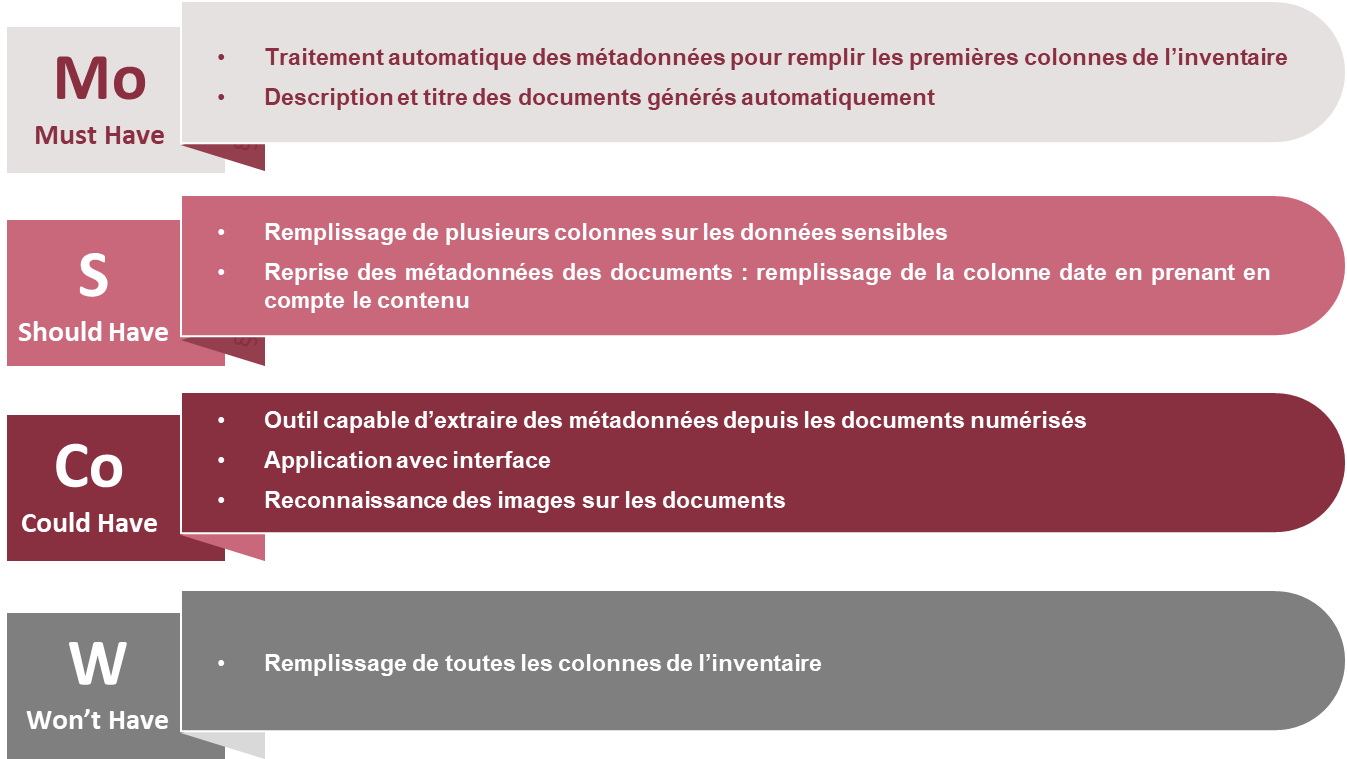
\includegraphics[width=\textwidth]{./media/image3.png}}
	\caption{Hiérarchisation des fonctionnalités à produire (MoSCoW) }
\end{figure}



Cette hiérarchisation a permis la réalisation du minimum requis. Lorsque
des difficultés sont apparues, les fonctionnalités non prioritaires ont
été mises de côté. Le projet InventAIre a ainsi démontré l'importance de
l'utilisation de méthodes de gestion de projets informatiques et d'une
bonne définition du périmètre. En effet,
l\textquotesingle ampleur des ressources et du personnel nécessaires à
la réussite des projets IA est souvent sous-estimée. Camille Girard-Chanudet évoque en parlant du
système basé sur le \emph{machine learning} développé à la Cour de Cassation
que «~loin de l'image d'autonomie généralement associée à ce type de
dispositifs techniques, la charge de travail humain dans le
fonctionnement d'un tel outil est conséquente~: celui-ci mobilise au
quotidien plus de 20 personnes à la Cour\footcite{girard-chanudet_travail_2023}~».
Le travail d'annotation des données à pseudonymiser demande en effet
beaucoup de ressources humaines. L\textquotesingle annotation en
\emph{machine learning} consiste à étiqueter ou décrire des données
(comme des images, du texte ou des sons) pour que les algorithmes
puissent apprendre à reconnaître et à traiter ces informations de
manière autonome. Cette étape est obligatoire pour le développement de modèles de \emph{machine
	learning} maison. En plus des personnes pour
réaliser les annotations, il faut également mobiliser du personnel pour
la gestion de projet et pour le développement de l'outil. Dans le cas du
projet InventAIre, nous n'avions pas le temps d'annoter des données
suffisantes pour développer un modèle d'IA en quatre mois de stage. Il
était donc impossible d'entraîner un modèle d'\gls{supervisé}. Nous avions ainsi 
comme option
l'\gls{non-supervisé} ou le choix d'un \gls{pré-entraîné}. Nous avons pu adapter le périmètre et
l'approche. Néanmoins, même dans le cas de l'usage de modèles
pré-entraînés, les investissements en temps et en ressources humaines
restent non-négligeables. Il faut par exemple prévoir une longue période
de tests afin de choisir le bon \gls{pré-entraîné} et mobiliser du personnel pour évaluer les résultats produits par l'IA. Pour un projet de
\gls{chatbot} à la BNL, d'après Yves Maurer, en charge du projet, le
«~plus chronophage a été de tester plusieurs alternatives pour chaque
brique du projet : des modèles de langage ouverts, un autre créé par
un groupe de recherche, celui de Meta et de Google\ldots \footcite{noauthor_comment_nodate}~». Dans le
	cadre de notre projet la période de tests a pris environ deux mois  avec une seule personne mobilisée. 

D'autres différences notables existent entre les projets archivistiques
et ceux impliquant l\textquotesingle IA. L\textquotesingle approche
cyclique est encore plus importante pour l\textquotesingle IA~: la
précision des outils produits doit
être évaluée à chaque étape. Les cycles sont de tailles différentes. Les
étapes de test et de réflexion sont assez lentes. Le code de l'outil en
lui-même a été assez rapide pour le projet InventAIre. Les périodes
d'évaluation et de reprise de l'outil en fonction des résultats de ces
dernières sont quant à elles longues et on ne peut pas prévoir leur nombre
d'itérations.\newline

\begin{center}
	Estimation du temps sur les différentes \enquote{tâches IA} pendant le projet
\end{center}

\begin{longtable}{|p{0.45\textwidth}|p{0.5\textwidth}|}

    \tableheader{Tâche}{Estimation de temps}
	
	Définition du périmètre et de l'approche & 15\% \\
	\hline
	Tests pour le choix d'un modèle & 40\% \\
	\hline
	Code sur l'intégration du modèle & 10\% \\
	\hline
	Prompt-engineering & 15\% \\
	\hline
	Évaluation de l'outil\up{*} & 15\% \\
	\hline
	Autre & 5\% \\
	\hline
\end{longtable}
\begin{noindentpar}
	\up{*}\footnotesize{Ce temps a été réduit parce que le stage se terminait, l'évaluation doit idéalement être plus longue pour être davantage pertinente et mener à des reprises de l'outil}
\end{noindentpar}\\

Un inconvénient de ces méthodes agiles est le temps que la gestion de
projet exige. Pendant notre stage, les tâches de gestion de projet ont
représenté environ 15 \% de notre temps\footnote{Un diagramme de répartition du	temps est consultable dans la note méthodologique en annexe.}, incluant
la définition du périmètre et du calendrier, la préparation et la tenue
des réunions ainsi que la rédaction des comptes rendus. Pour des
projets de plus grande envergure, il est essentiel de séparer les
fonctions de recherche et développement de celles de gestion de projet
entre plusieurs personnes. La constitution d'une équipe projet
favorisant la collaboration entre archivistes et spécialistes des
technologies de l'information est nécessaire.

Enfin, ces projets nécessitant d'importants investissements humains et
financiers et l'intelligence artificielle étant un nouveau territoire à
explorer pour les institutions publiques, il est nécessaire de commencer
par des projets pilotes, des preuves de concept (POC) ou des études de
faisabilité avant de se lancer dans de grands projets. La plupart des
institutions suivent ces recommandations. C'est notamment le cas de la
BNL (Bibliothèque nationale du Luxembourg) qui a lancé plusieurs projets pilotes ces dernières années, dont un
projet d'amélioration de la transcription par \gls{OCR} et un projet de \emph{chatbot} permettant la recherche
dans les fonds de presse numérisés\footcite{noauthor_comment_nodate}. À la Chambre des Députés, le projet InventAIre constitue
la première étape d\textquotesingle un processus plus large. La phase
suivante consiste à réaliser un POC, à partir duquel un outil serait
développé et mis en production.

L\textquotesingle intégration des méthodes de gestion de projet, en
particulier les approches agiles, est par conséquent une composante de la réussite des
projets IA dans le secteur des archives. Le projet InventAIre illustre
comment une gestion efficace, une collaboration interdisciplinaire et
une approche itérative permettent d'être en mesure de naviguer avec succès entre les défis spécifiques à l\textquotesingle IA.

\subsection{Gestion des risques et défis éthiques des systèmes	basés sur le \emph{machine learning}}

Les risques liés à l\textquotesingle intelligence artificielle, en
particulier dans le domaine des archives, sont nombreux, allant bien
au-delà des simples considérations légales facilement identifiables.
Outre les enjeux juridiques, il existe des risques sociaux et
éthiques, qui seront détaillés dans le début du chapitre 8. Face à ces défis,
une analyse de risques est à prévoir. A la Chambre des Députés, une
mitigation des risques a été réalisée en amont en collaboration avec le
\emph{DPO (data protection officer)} et le Responsable sécurité des
systèmes informatiques. C'est ainsi qu'il a été décidé qu'il n'était pas
question de transmettre des données à un tiers, nous avons ainsi dû
travailler avec des modèles pré-entraînés hébergés localement sur nos
ordinateurs, et non dans le \emph{cloud}. Cela n'est pas sans conséquence. Ceux
que nous pouvions faire tourner étaient en effet moins précis que les
grands modèles hébergés dans le \emph{cloud} et très volumineux sur nos
machines, donc relativement lents. Les autres risques identifiés
concernaient un mauvais remplissage de l'inventaire, contenant des biais
ou \gls{hallucination}s. Les titres et descriptions en texte libre générés par
des grands modèles de langage peuvent facilement contenir des
erreurs, des informations non pertinentes ou des hallucinations. Au
contraire l\textquotesingle IA pourrait aussi invisibiliser certaines
informations jugées non pertinentes, entraînant une perte de données
essentielles. Enfin, la gestion des données sensibles nécessite une
attention particulière : une erreur dans ces données pourrait avoir des
conséquences graves. Face à ces risques, il a été décidé qu'un contrôle
qualité rigoureux serait effectué. 
Un tableau contenant les risques et contre-mesures identifiés au début du projet se trouve dans la partie 1.1.2. de la note méthodologique en annexe.\newline

Le chercheur James Lappin propose dans sa thèse intitulée «~The science
of recordkeeping systems -- a realist perspective~», une distinction
entre les applications «~low-stakes~» (à faible enjeu) et
«~high-stakes~» (à fort enjeu) de l'IA dans le domaine du \emph{record
	management}. Les applications « low-stakes » incluent
l\textquotesingle utilisation de l\textquotesingle IA pour classer les
résultats de recherche, personnaliser les recommandations, visualiser
les contenus ou extraire des entités, sans altérer les règles
d\textquotesingle accès ou de conservation des documents. En revanche,
les applications « high-stakes » impliquent des décisions aux
conséquences irréversibles, qui modifient les règles de conservation ou
d\textquotesingle accès aux documents, par exemple via des éliminations ou
l\textquotesingle octroi de certains accès\footcite{lappin_science_2024}. Les autres projets
d\textquotesingle intelligence artificielle mis en place dans le domaine
des archives et des bibliothèques au Luxembourg sont majoritairement des
projet «~low-stakes~». C'est par exemple le cas des \emph{chatbots} de la
Bibliothèque Nationale du Luxembourg (BNL) et du Parlement européen
mentionnés précédemment, qui permettent une recherche dans des documents
publics. Quant aux scripts générés par IA des ANLux, ils ont vocation à être
partagés, c'est aussi une utilisation avec moins de risques, car sans données confidentielles. 

Le projet
InventAIre est précurseur en termes d'application
«~high-stake~» de traitement automatique d'archives par IA. Il a ainsi constitué
une occasion de tirer plusieurs enseignements précieux concernant la
gestion des risques et leur atténuation. D\textquotesingle abord, il est
apparu particulièrement intéressant d\textquotesingle impliquer divers
acteurs dans le processus, tels que le responsable de la sécurité des
systèmes informatiques (RSSI) et le \emph{data protection officer} (DPO). Ces experts dans leur domaine
apportent des compétences spécifiques complémentaires à celles des
archivistes et des informaticiens. De plus, nous avons cherché à
impliquer le plus possible l'humain. C'est le concept de l'«~Human in
the loop~»~: l\textquotesingle humain a été intégré dans le processus de
développement et d\textquotesingle évaluation de l\textquotesingle IA.
Cela est particulièrement pertinent et à développer dans le cadre des
sprints agiles mentionnés précédemment, où chaque étape du développement
était validée par des retours humains. Cette méthode contribue non seulement à une meilleure
qualité des résultats, mais facilite également
l\textquotesingle instauration d\textquotesingle une meilleure confiance
des différents acteurs impliqués envers l'outil développé. Cette dernière facilite la \gls{changement}.
L\textquotesingle analyse des risques a joué un rôle dans la
construction de cette confiance en garantissant que chaque décision
prise soit justifiée. Cela a permis de créer un cadre sécurisé et le
plus transparent possible, favorisant ainsi l\textquotesingle adoption
et l\textquotesingle acceptation de l\textquotesingle IA dans un domaine
aussi sensible que celui des archives.

Les projets d'intelligence artificielle dans le domaine des archives
publiques offrent des perspectives prometteuses, mais ils posent
également des défis importants. Avant d'initier de tels projets, il convient
d'assurer une analyse des risques de manière proactive. Les exigences
éthiques et techniques sont nombreuses. Les besoins et usages doivent
être clairement identifiés et la gestion de projet réfléchie. \newline

En conclusion de ce chapitre, nous pouvons dire que les producteurs d\textquotesingle archives publiques luxembourgeois font
face à de nombreux défis qui, paradoxalement, offrent des opportunités
d\textquotesingle innovation et d\textquotesingle expérimentation. Un
contexte favorable au Luxembourg et en Europe encourage
l\textquotesingle implémentation de projets IA dans le secteur public
avec des ambitions élevées. Cependant, avant de lancer de tels projets,
des réflexions sur les prérequis en termes de pilotage sont à mener. Une
fois ces réflexions approfondies, les projets IA pourront aboutir à des
résultats et avoir des apports concrets pour les services
d\textquotesingle archives publics.